\documentclass[11pt]{scrartcl}
\usepackage[sexy]{evan}
\usepackage{graphicx}
\usepackage[spanish]{babel}
\graphicspath{ {./images/} }

\usepackage{answers}
\Newassociation{hint}{hintitem}{all-hints}
\renewcommand{\solutionextension}{out}
\renewenvironment{hintitem}[1]{\item[\bfseries #1.]}{}

\usepackage{venndiagram,multicol,hyperref,graphicx,array,xskak}
\usepackage{tikz}
\usetikzlibrary{positioning,trees}

\begin{document}
\title{Combinatoria Sucesiones}
\author{Ricardo Largaespada}
\date{24 Agosto 2024}

\maketitle

\section{Introducción}

En esta clase, aplicaremos muchas de las ideas que aprendimos durante este curso para resolver problemas sobre sucesiones. Como ocurrió en la clase de Combinatoria Geométrica, ten siempre en mente los principios del palomar, del extremo y de la invariancia. Pero también no olvides usar inducción siempre que esto parezca útil. Sin embargo, comenzaremos la clase con un problema de conteo.

\begin{example}
Determina la cantidad de diferentes permutaciones $a_1, a_2, \dots, a_{10}$ de los enteros $1, 2, \dots, 10$ tales que $a_i > a_{2i}$ ($1 \leq i \leq 5$) y $a_i > a_{2i+1}$ ($1 \leq i \leq 4$).
\end{example}
\textbf{Solución.} Primero, sustituye las desigualdades del problema por el siguiente diagrama:
\begin{center}
    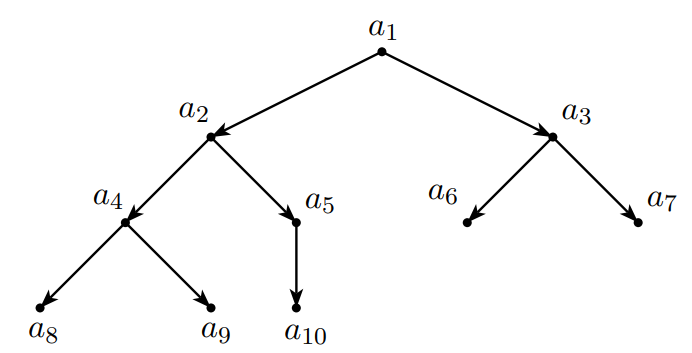
\includegraphics[scale=.75]{images/clase_14-orden-secuencia.png}
\end{center}

El diagrama está construido de forma que la relación $a_i \rightarrow a_j$ indica que $a_i > a_j$. Por la figura, queda claro que debemos tener $a_1 = 10$. De los 9 enteros restantes, debemos escoger tres de ellos para formar el conjunto $\{a_3, a_6, a_7\}$. Hecho esto, $a_3$ debe ser el mayor de ellos, y el orden entre $a_6$ y $a_7$ no debe importar. Por lo tanto, tenemos 
\[
\binom{9}{3} \times 2
\]
posibilidades para los números $a_3, a_6, a_7$ del diagrama.

Hasta ahora hemos escogido la posición de cuatro números. Los seis restantes formarán parte del conjunto $\{a_2, a_4, a_5, a_8, a_9, a_{10}\}$. Observa que en esta situación, $a_2$ debe ser el mayor de los seis enteros restantes. Además, de los cinco que quedarán, después de fijar $a_2$, debemos escoger tres para formar el conjunto $\{a_4, a_8, a_9\}$. De estos tres, $a_4$ debe ser el mayor y el orden entre $a_8$ y $a_9$ no debería importar. Entonces, tendremos 
\[
\binom{5}{3} \times 2
\]
posibilidades para el conjunto $\{a_4, a_8, a_9\}$.

Finalmente, los dos números restantes serán $a_5$ y $a_{10}$, siendo $a_5$ el mayor entre estos dos. Por lo tanto, tenemos
\[
\binom{9}{3} \times 2 \times \binom{5}{3} \times 2 = 3360
\]
permutaciones con las propiedades requeridas.

\begin{example}
Encuentra el mayor valor posible de la expresión
\[
x_1x_2 + x_2x_3 + \cdots + x_nx_1
\]
para $n \geq 3$, donde $x_1, x_2, \dots, x_n$ es una permutación arbitraria de los enteros $1, 2, \dots, n$.
\end{example}
\textbf{Solución.} Sea $S_n(x_1, \dots, x_n) = x_1x_2 + x_2x_3 + \dots + x_nx_1$ la función anterior y $M_n$ su valor máximo. Como $S_n$ es invariante por permutaciones cíclicas, podemos escoger aquella en la que $x_1 = n$. Observa que
\begin{align*}
S_n(n, x_2, \dots, x_n) &= S_{n-1}(x_2, \dots, x_n) - x_2x_n + nx_2 + nx_n \\
&= S_{n-1}(x_2, \dots, x_n) + n^2 - (n - x_2)(n - x_n)
&\leq M_{n-1} + n^2 - 1 \cdot 2
\end{align*}

en la cual en la primera igualdad usamos la definición de $S_n$, en la segunda simplemente reescribimos $x_2x_n + nx_2 + nx_n$ y en la tercera maximizamos el término $-(n - x_2)(n - x_n)$ y usamos la definición de $M_{n-1}$.

Haciendo una suma telescópica, tenemos
\begin{align*}
M_n &\leq M_3 + (4^2 - 2) + (5^2 - 2) + \dots + (n^2 - 2) \\&= 11 + (4^2 + 5^2 + \dots + n^2) - 2(n - 3) \\&= \frac{1}{6}(2n^3 + 3n^2 - 11n + 18).
\end{align*}
Dejamos al lector la verificación de que la cota obtenida es realmente óptima.

\begin{example}[Cono Sur 2012] Alrededor de una circunferencia están escritos 2012 números, cada uno de ellos es igual a $1$ o $-1$. Si no hay 10 números consecutivos cuya suma sea $0$, encuentra todos los valores posibles de la suma de los 2012 números.
\end{example}
\textbf{Solución.} Sean $a_1, a_2, \dots, a_{2012}$ los números escritos en la circunferencia. Sea $S_i$ la suma de diez números consecutivos comenzando a partir de $a_i$. Observa que cada $S_i$ debe ser un número par, ya que es la suma de diez números impares. Observa que $|S_i - S_{i+1}| \in \{0, 2\}$. Ahora supongamos que existen $i$ y $j$ tales que $S_i$ y $S_j$ poseen signos diferentes. Por una propiedad del valor intermedio, debe existir algún $k$ entre $i$ y $j$ tal que $S_k = 0$.

Por lo tanto, asumiremos sin pérdida de generalidad que todos los $S_i$ son positivos. En este caso,
\[
S_1 + S_2 + \dots + S_{2012} \geq 2012 \times 2 = 4024
\]
En la suma anterior, cada $a_i$ se cuenta exactamente 10 veces. Luego, la suma de todos los números en la circunferencia debe ser al menos 404. El primer número par que satisface esta cota es 404. Observa que es posible obtener este valor repitiendo la secuencia de bloques $1, 1, 1, 1, 1, 1, -1, -1, -1, -1$ a partir de $a_i$. Y cada par entre 404 y 2012 (incluyendo 2012) se obtiene intercambiando un $(-1)$ por un $(1)$ en la configuración. Mientras que los números negativos se obtienen intercambiando los signos de todos los números de una configuración.

\begin{example}[Rusia]
Sean $a_1, a_2, \dots, a_m$, $b_1, b_2, \dots, b_n$ reales positivos tales que
\[
a_1 + a_2 + \dots + a_m = b_1 + b_2 + \dots + b_n.
\]
En un tablero vacío de $m$ filas y $n$ columnas se deben escribir números no negativos de modo que la suma de los números en la $i$-ésima fila sea igual a $a_i$ y la suma de los números en la $j$-ésima columna sea igual a $b_j$ ($1 \leq i \leq m$, $1 \leq j \leq n$). Muestra que es posible obtener tal configuración usando a lo sumo $m + n - 1$ números positivos.
\end{example}
\textbf{Solución.} Considera un segmento de tamaño $a_1 + a_2 + \dots + a_m$ dividido en $m$ segmentos de tamaños $a_1, a_2, \dots, a_m$. Llamaremos a $A_i$ el segmento de longitud $a_i$.
\begin{center}
    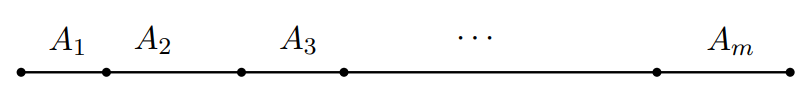
\includegraphics[scale=.75]{images/clase_14-rusia1.png}
\end{center}
Considera también un segmento de tamaño $b_1 + b_2 + \dots + b_n$ dividido en $n$ segmentos de tamaños $b_1, b_2, \dots, b_n$. Llamaremos a $B_i$ el segmento de longitud $b_i$.
\begin{center}
    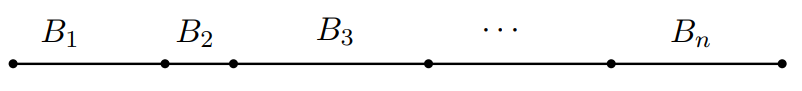
\includegraphics[scale=.75]{images/clase_14-rusia2.png}
\end{center}
Los dos segmentos anteriores tienen la misma longitud, ya que \(a_1 + a_2 + \cdots + a_m = b_1 + b_2 + \cdots + b_n\). Por lo tanto, superponiendo estos segmentos obtendremos un tercero que tendrá la misma longitud y se dividirá como máximo en \(m + n - 1\) subdivisiones. Por último escribiremos el tamaño del segmento en la casilla de la fila \(i\) y la columna \(j\) del tablero \(A_i \cap B_j\). Y si esta intersección está vacía, escribimos 0.

\begin{example}
Sean \( a_1, a_2, \dots, a_n \) y \( b_1, b_2, \dots, b_n \) dos permutaciones del conjunto de números \( 1, \frac{1}{2}, \frac{1}{3}, \dots, \frac{1}{n} \) tales que  
\[
a_1 + b_1 \geq a_2 + b_2 \geq \cdots \geq a_n + b_n.
\]  
Demuestra que la desigualdad \( a_k + b_k \leq \frac{4}{k} \) se cumple para todo \( k = 1, 2, \dots, n \).
\end{example}
\textbf{Solución:}  
Fijemos un índice \( k \) cualquiera. Supongamos que en el conjunto de índices \( \{1, 2, \dots, k\} \) la desigualdad \( a_j \leq b_j \) ocurre \( x \) veces, mientras que la desigualdad \( a_j \geq b_j \) ocurre \( y \) veces. Como \( x + y \geq k \), asumamos sin pérdida de generalidad que \( x \geq \frac{k}{2} \). Definamos \( b_s \) como el menor entre los \( b_j \) tales que \( a_j \leq b_j \). Observe que debemos tener \( b_s \leq \frac{1}{x} \), ya que \( b_j \geq b_s \) ocurre al menos \( x \) veces. De esta forma,  
\[
a_k + b_k \leq a_s + b_s \leq 2b_s \leq \frac{2}{x} \leq \frac{2}{k/2} = \frac{4}{k}.
\]

\Opensolutionfile{all-hints}
\section{Problemas Propuestos}

\begin{problem}
Diagramas como el elaborado en el primer problema son conocidos como Diagramas de Hasse para conjuntos parcialmente ordenados. En este ejercicio, debes responder la siguiente pregunta: Dado un diagrama de Hasse con \( n \) vértices, ¿cuántas de las permutaciones de \( 1, 2, \dots, n \) satisfacen el orden parcial dado por ese diagrama? Analiza los siguientes casos:
\begin{center}
    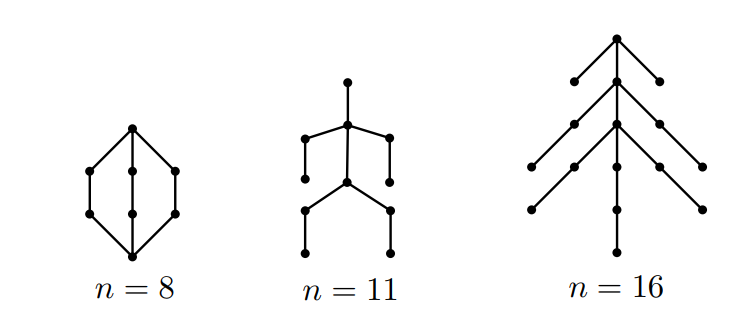
\includegraphics[scale=.75]{images/clase_14-hasse.png}
\end{center}
\begin{hint}
Para abordar este problema, considera primero el caso simple de \( n = 3 \) o \( n = 4 \) y verifica cómo las permutaciones se ajustan al diagrama de Hasse. Trata de establecer una relación entre el número de permutaciones y el número de vértices en el diagrama.
\end{hint}
\end{problem}

\begin{problem}
Existen números reales no negativos \( a_1, a_2, \dots, a_7 \) tales que \( a_1 = a_7 = 0 \) y al mismo tiempo \( a_{i+1} + a_{i-1} > a_i \sqrt{3} \) para \( 2 \leq i \leq 6 \)?
\begin{hint}
    Para resolver este problema, considera probar valores específicos para \( a_i \) y verifica si puedes encontrar una configuración que cumpla con las desigualdades dadas. Un enfoque es probar valores como \( a_i = 0 \) o valores pequeños positivos para analizar el cumplimiento de las desigualdades.
\end{hint}
\end{problem}

\begin{problem}
Encuentra el mayor valor posible de la suma
\[
S = |x_1 - 1| + |x_2 - 2| + \cdots + |x_n - n|,
\]
donde \( x_1, x_2, \dots, x_n \) es una permutación de \( 1, 2, \dots, n \).
\begin{hint}
    Considera el caso de \( n = 3 \) o \( n = 4 \) para ver cómo se puede maximizar la suma \( S \). Analiza las permutaciones posibles y cómo cada una contribuye a la suma total. Para generalizar, piensa en cómo el valor de \( S \) cambia con el tamaño de la permutación y busca un patrón.
\end{hint}
\end{problem}

\begin{problem}
Supón que existe una secuencia infinita de números reales \( x_1, x_2, \dots \) tal que para cualesquiera índices \( m, n \) tenemos
\[
|x_{m+n} - x_n - x_m| < \frac{1}{m + n}.
\]
Muestra que esta secuencia es una progresión aritmética.
\begin{hint}
    Considera cómo la diferencia \( x_{m+n} - x_n - x_m \) se comporta cuando \( m \) y \( n \) toman valores grandes. Utiliza la definición de una progresión aritmética y demuestra que la secuencia debe tener una diferencia constante para satisfacer la condición dada.
\end{hint}
\end{problem}

\Closesolutionfile{all-hints}

\section{Sugerencias y Soluciones}
\begin{enumerate}
\input{all-hints.out}
\end{enumerate}

\end{document}